\subsection{Aufzeichnung}

In diesem Abschnitt geht es um die Wandlung von analogen zu digitalen Signalen (und umgekehrt). Hierbei werden die Klänge durch eine Sinuskurve dargestellt.
\notebox{Bei der Digitalisierung von Klängen gibt es eine Regel die immer beachten werden muss. Die Abtastrate muss mindesten 2x so hoch sein wie die Originalquelle. Der Mensch hört maximal bis zu 20.000Hz, das bedeutet die Abtastrate muss über 40.000 Hz betragen, also 40.001. Üblich ist jedoch 44.100 (CD) und sonst eigentlich 48.000Hz oder ein vielfaches davon.
Wenn dies nicht geschieht (unterabtastung) entstehen neue Schwingungen die im Orhinal nicht vorhanden waren.} 
\paragraph{A/D Wandlung}~
\begin{figure}[h]
    \centering
    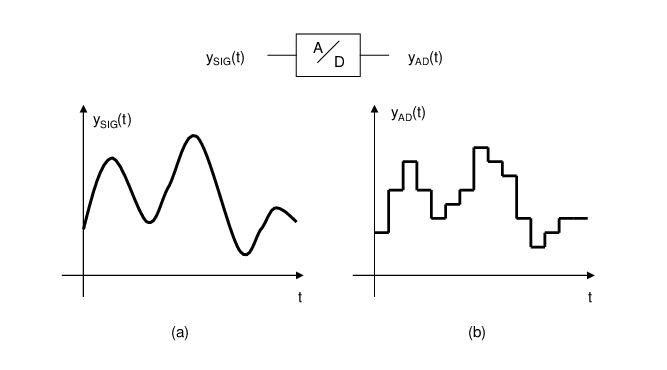
\includegraphics[width=0.8\linewidth]{Bilder/Medientechnik/DA-Wandlung.png}
    \caption{Analog / Digital Wandlung \cite{DA-Wandlung:online}}
    \label{fig:AD-Wandlung}
\end{figure}

Bei der Analog zur Digitalwandlung wird ein Analoges Signal in Form einer Welle aufgenommen und abgetastet. Dann wird in Regelmäßigen Abstanden (z.B. 48.000x pro Sekunde) abgetast. Von der Welle ausgehend wird dann der Wert zum nächsten "Bit" angehoben oder abgesenkt um dann entsprechend eine Spannungskirve zu erzeugen. Im Bild rechts ist dies zu sehen. Jedem dieser Platos wird entsprechend ein Bitwert zugewiesen, die Bitrate (z.B. 16Bit) gibt dann an wie viele von diesen Platos es gibt. 
\cite{DA-Wandlung:online}

\textbf{Eine genauere Erklärung sind in den Unterlagen von Matthias Reusch}

